\section{Datasets}

\setLayout{mainpoint}

\begin{frame}[noframenumbering, plain]{}
    \frametitle{Datasets}
\end{frame}

\setLayout{vertical}

%---------------------------------------------------------
\begin{frame}{Available Datasets}

    \begin{itemize}
        \item Majority of related works acquired their own images.
        \item The work of Lacalle et al.
    \end{itemize}

    \begin{table}[]
        \centering
        \setlength{\tabcolsep}{10pt}
        
        {\rowcolors{2}{}{LightGray!10}
            \begin{tabular}{lcccccc}
                \textbf{Name} & \textbf{BL5S} & \textbf{BN2S} & \textbf{BN10S} & \textbf{FL5C} & \textbf{FL5S} & \textbf{FN2S} \\
                \midrule
                Method & Brif & Brif & Brif & Fluo & Fluo & Fluo \\
                Images & 50 & 154 & 105 & 19 & 50 & 34 \\
                Magnification & 5x & 2x & 10x & 5x & 5x & 2x \\
                Culture & Susp & Susp & Susp & Colla & Susp & Susp
            \end{tabular}
        }
    \end{table}
\end{frame}

%---------------------------------------------------------
\begin{frame}{Lacalle et al. annotations}
    \begin{itemize}
        \item Annotated via ImageJ software.
        \item ImageJ only saves the vertices.
        \item Python script to generate mask images.
    \end{itemize}
\end{frame}

%---------------------------------------------------------
\begin{frame}{Samples from Lacalle et al.}
    \begin{figure}[!htb]
        \centering
        \subfloat{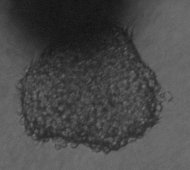
\includegraphics[width=3cm, height=3cm]{figures/datasets/1}}
        \subfloat{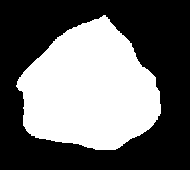
\includegraphics[width=3cm, height=3cm]{figures/datasets/1_mask}}\hspace*{0.1cm}
        \subfloat{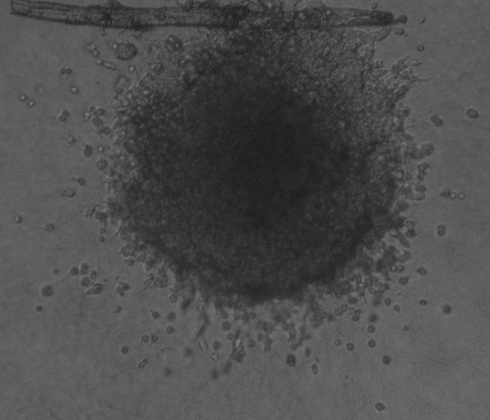
\includegraphics[width=3cm, height=3cm]{figures/datasets/11}}
        \subfloat{
\includegraphics[width=3cm, height=3cm]{figures/datasets/11_mask}}\\
        \subfloat{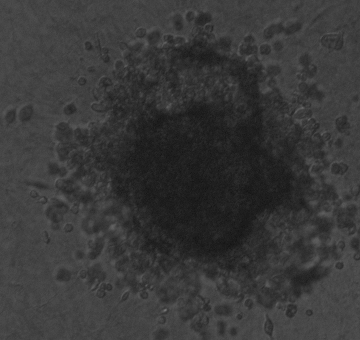
\includegraphics[width=3cm, height=3cm]{figures/datasets/7}}
        \subfloat{
\includegraphics[width=3cm, height=3cm]{figures/datasets/7_mask}}\hspace*{0.1cm}
        \subfloat{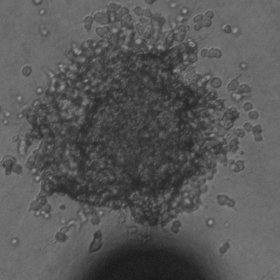
\includegraphics[width=3cm, height=3cm]{figures/datasets/6}}
        \subfloat{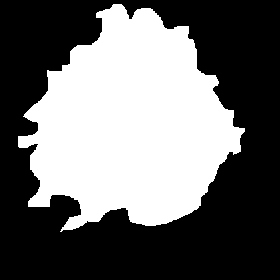
\includegraphics[width=3cm, height=3cm]{figures/datasets/6_mask}}
    \end{figure}
\end{frame}

%---------------------------------------------------------
\begin{frame}{Proposed Datasets}
    \begin{itemize}
        \item OncoBiomarkers Research Laboratory at UNICAMP;
            %\begin{itemize}
                %\item Professor Carmen Veríssima Ferreira;
            %\end{itemize}
        \item Two images per spheroid;
    \end{itemize}
\end{frame}

%---------------------------------------------------------
\setLayout{horizontal}

\begin{frame}{Spheroid Acquisition}
    \begin{figure}
        \centering
        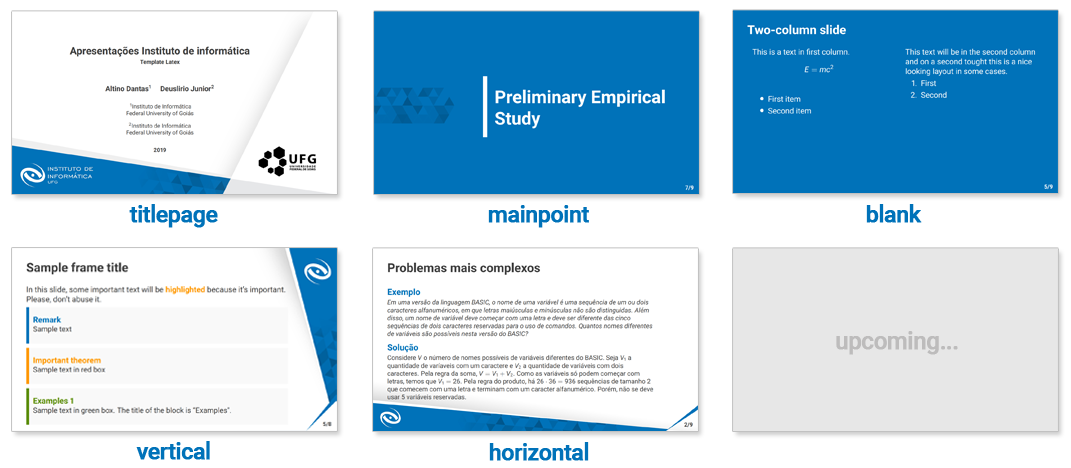
\includegraphics[width=.9\textwidth]{readme/layouts.png}
    \end{figure}
\end{frame}

%---------------------------------------------------------
\begin{frame}{Image Acquisition}
    \begin{figure}[!htb]
        \centering
        \subfloat[$48$h]{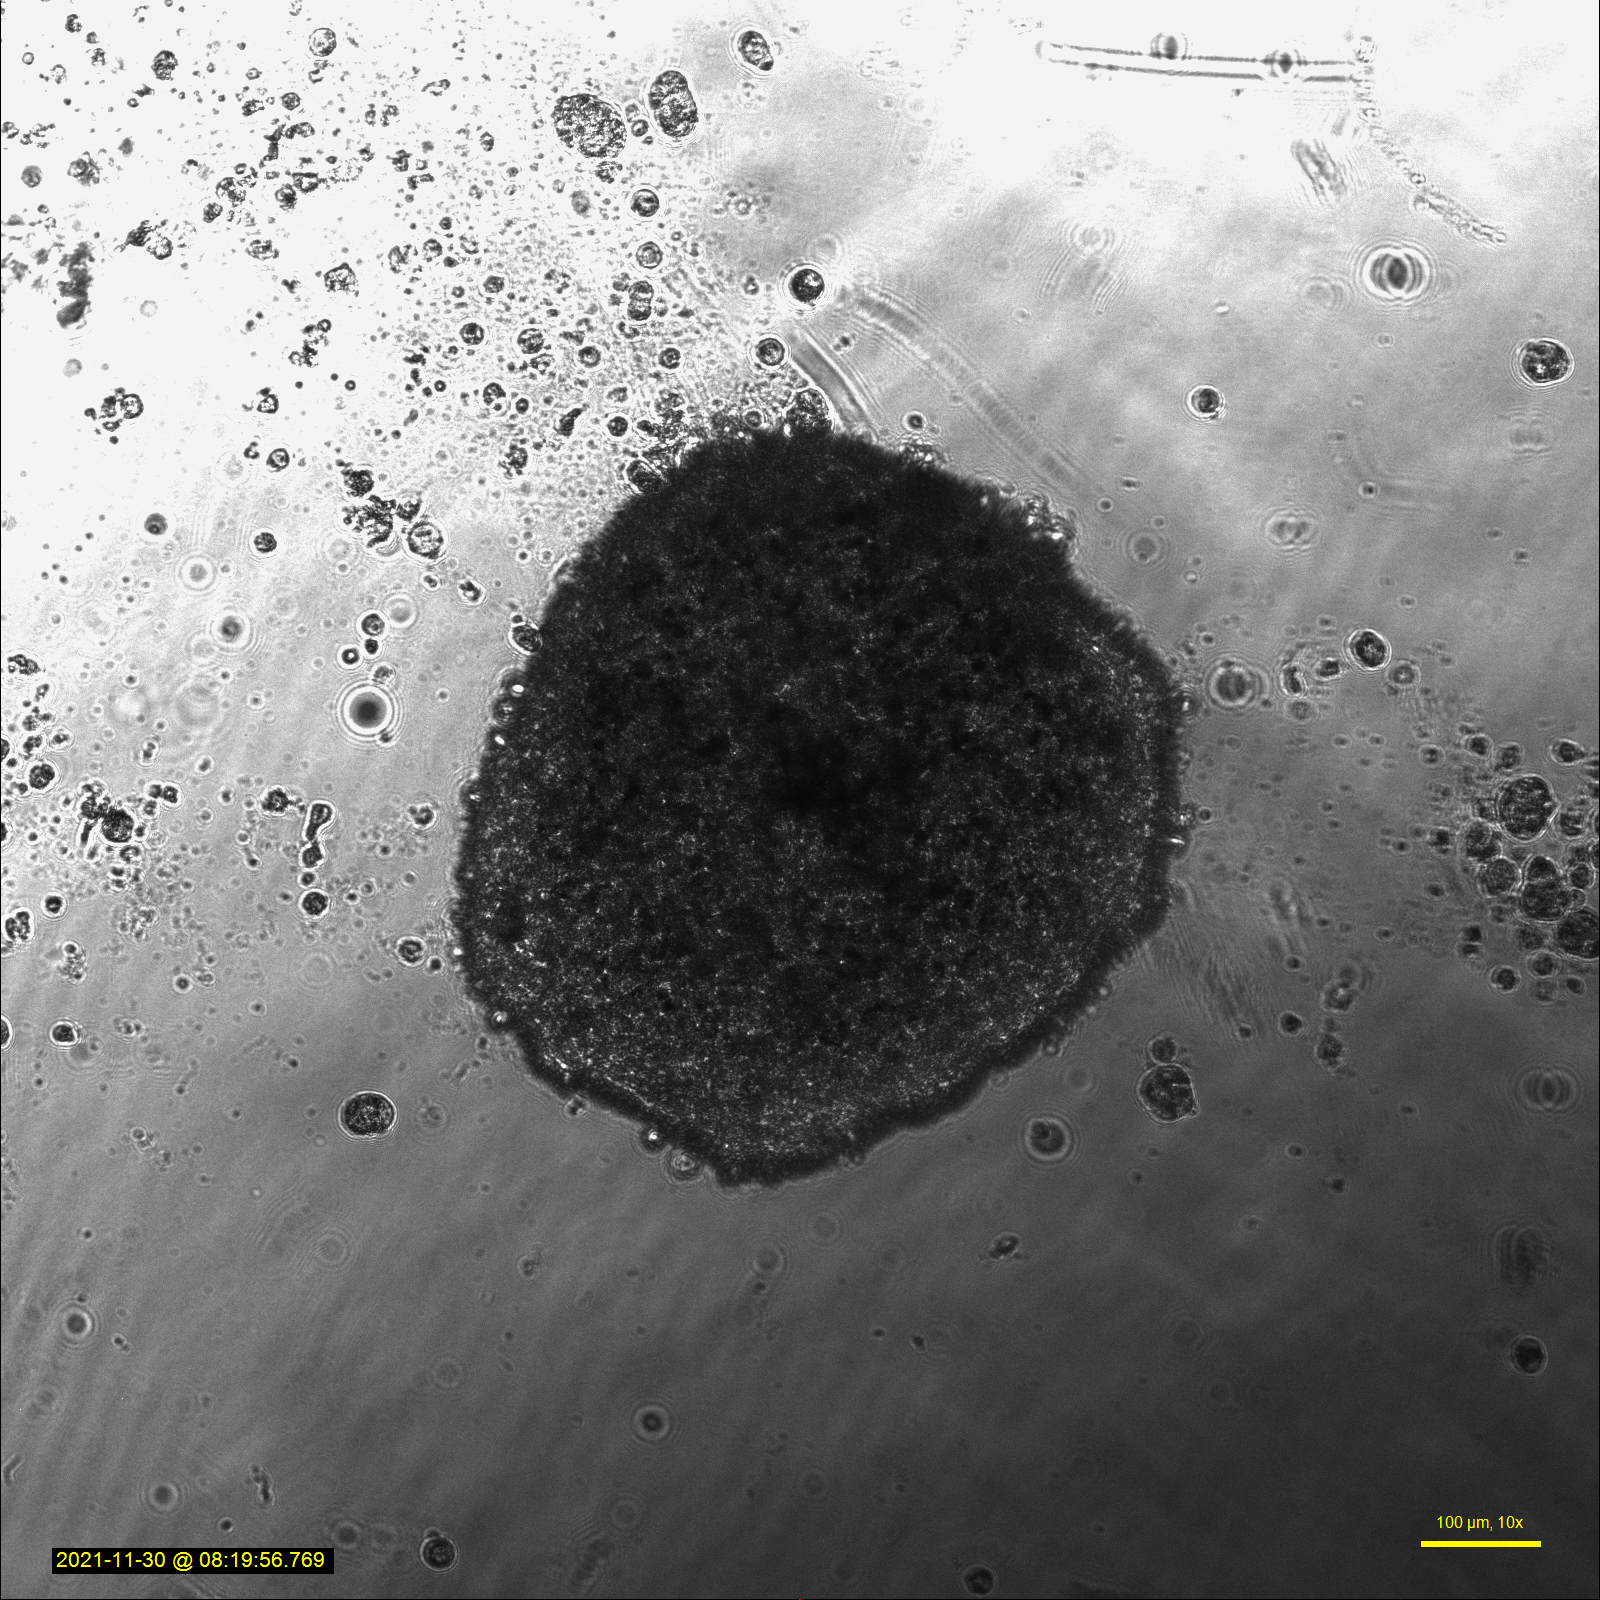
\includegraphics[width=4cm]{figures/datasets/48_B12N}}
        \subfloat[$72$h]{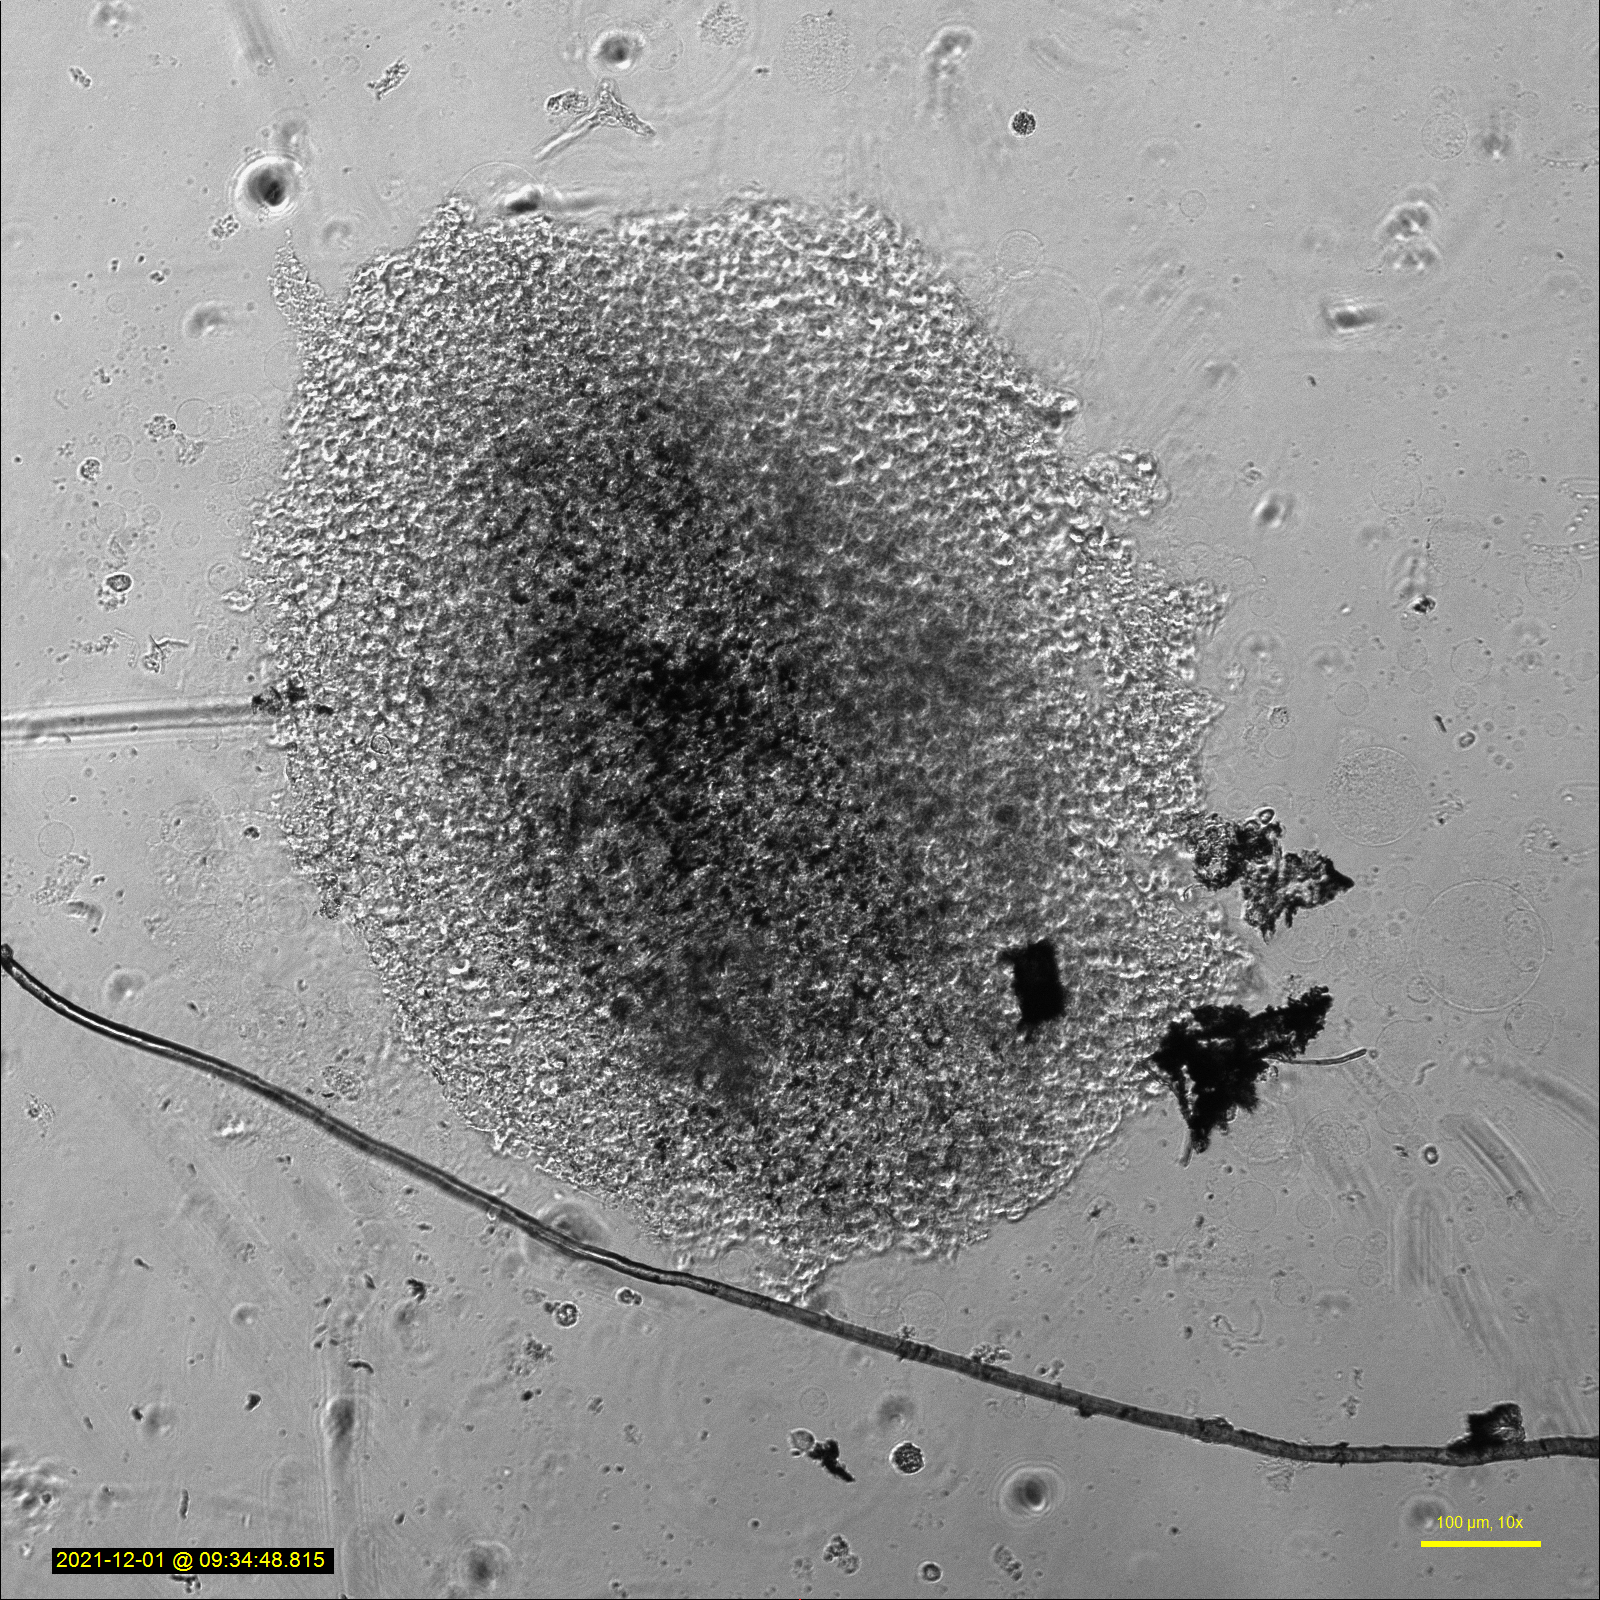
\includegraphics[width=4cm]{figures/datasets/72_B12N}}
        \subfloat[$96$h]{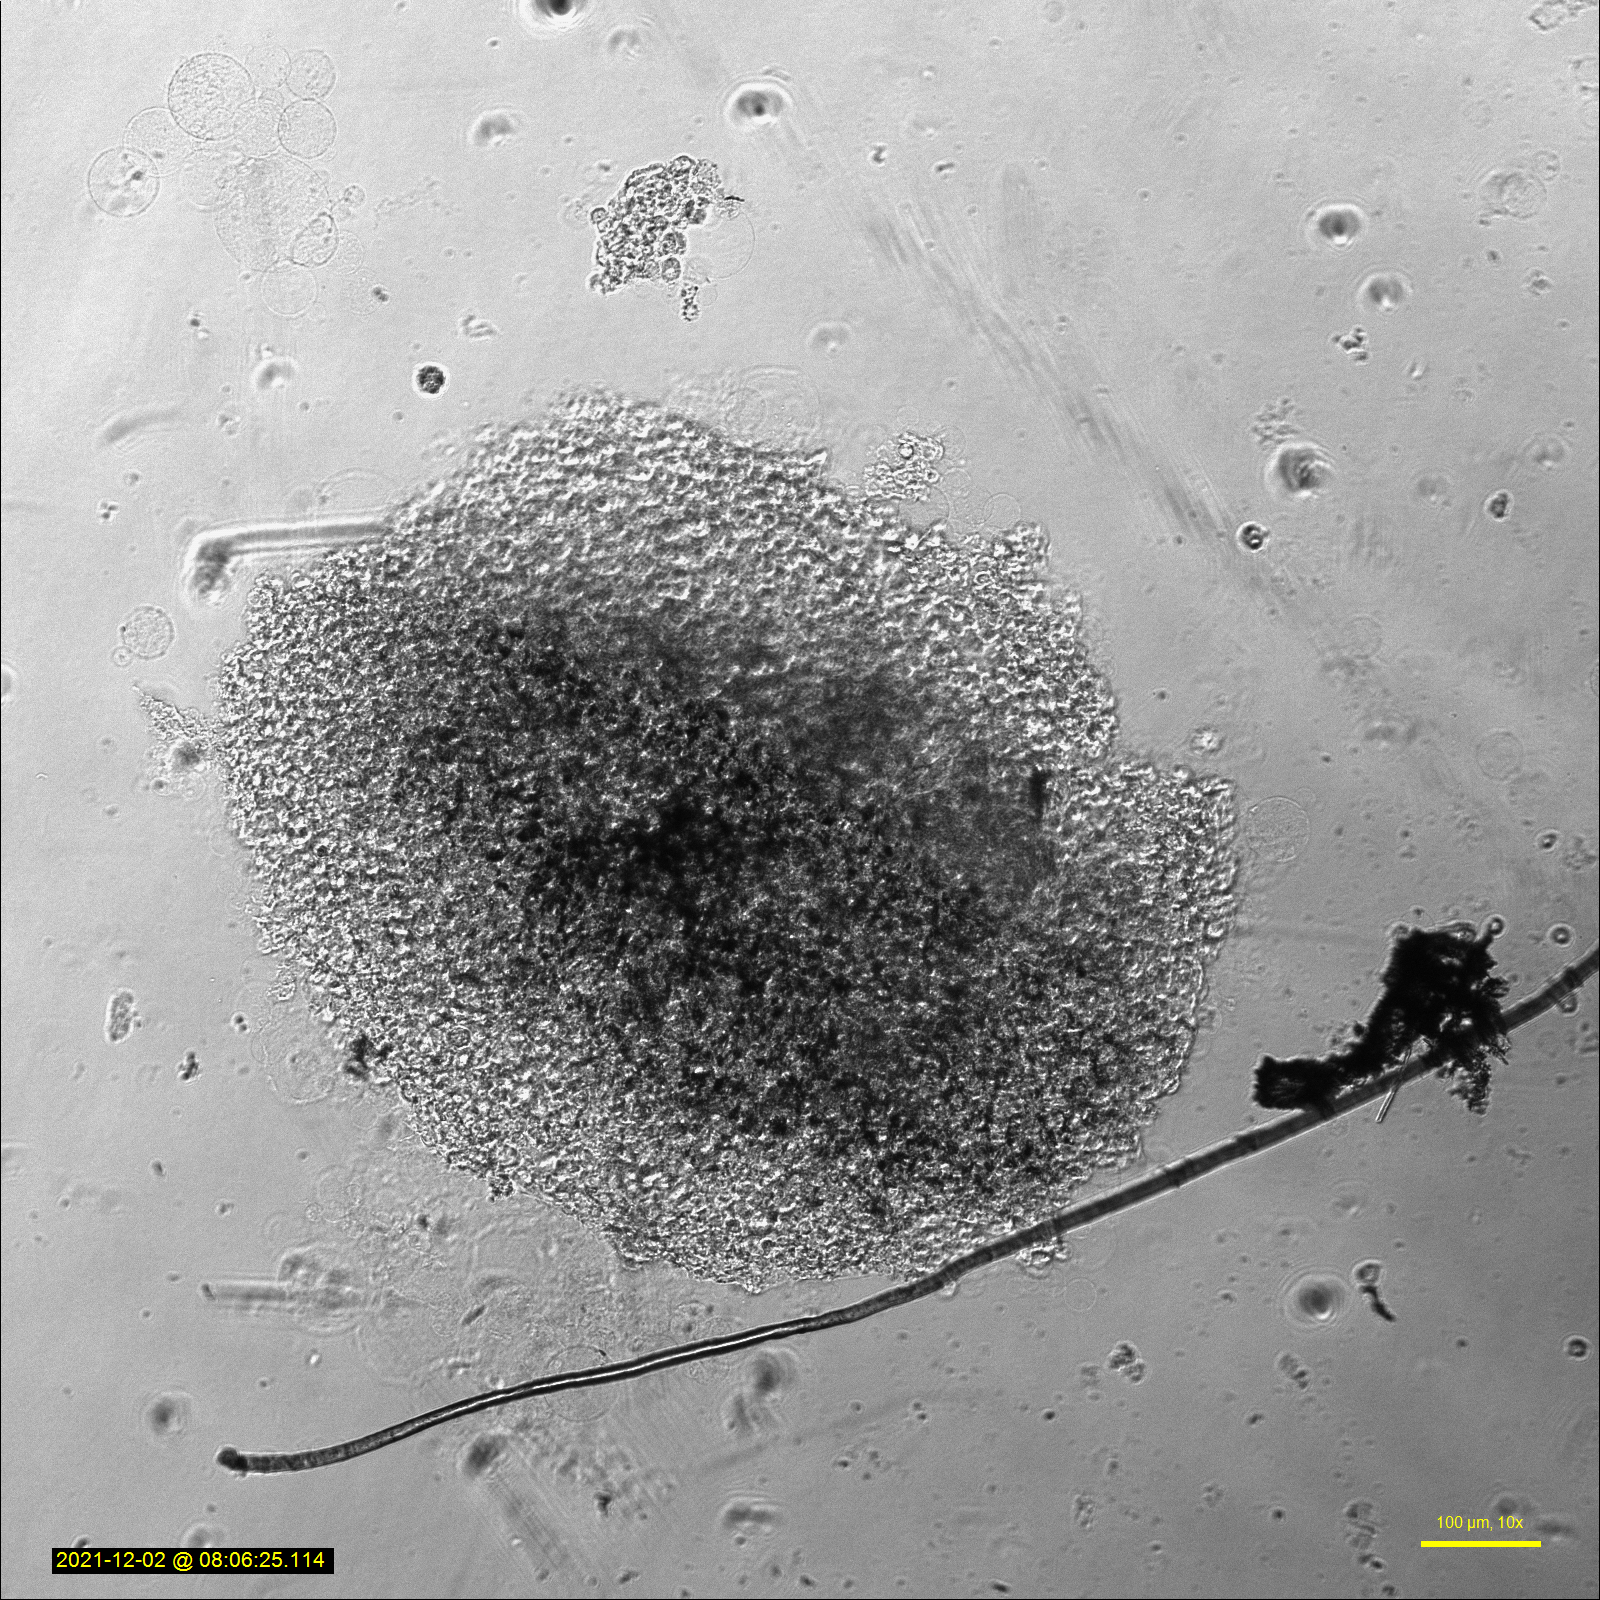
\includegraphics[width=4cm]{figures/datasets/96_B12N}}
    \end{figure}
\end{frame}
